The members of the C2 System interacts with each other, exchanging information and awareness, and the variables evolved in these operations with all conditional rules need to be formalized. The representation chosen, called Program Graph (PG), is applied over a set of typed variables and it is represented by the following tuple:

\begin{center}
    $(Loc,Act,Effect,\lhookrightarrow,Loc_0,g_0)$
\end{center}

where,

\begin{itemize}
	\item $Loc$ is a set of location  
	\item $Act$ is a set of actions
	\item Effect is a function defined by $Act \times Eval(Var) \to Eval(Var)$
	\item $\lhookrightarrow$ is the conditional transition relation defined by $Loc \times Cond(Var) \times Act \times Loc$
	\item $Loc_0 \subseteq Loc$ is the set of initial locations
	\item $g_0 \in Cond(Var)$ is the initial condition
\end{itemize}


This representation applies conditional rules, actions and map effects over these variables, conducting the system or entity to different states. \cite{baier}. Our basic element, i.e., the DSPL, had its states modelled with this technique.

As the C2 Domain deals with dynamic context and it is under the effects of changes in the circumstances, the element representation needs to operate with variables that represents this circumstance and its dynamism. Based on the domain studies, these changes can be classified in three categories: self, environment and mission.

The pair formed by the element status ($E$) and the list of tasks allocated ($T$) represent all those changes categories. According to the mission change, the list of tasks allocated can change, adding or removing tasks from it. The sensors on board are able to obtain new conditions from the environment and its possible changes. Besides that, the element $E$ (DSPL) is represented by its feature model ($FM$) that groups all possible valid configurations that it can get during the execution. It represents the changes in the self.

Basically, the element $E$ assumes a valid configuration $c \in \llbracket FM \rrbracket$ and it has a set of tasks ($T$) allocated to be performed. The system is represented by three roles: C2 Approach Selector (C2A), Task Allocator (TA) and Executor (EX). Its execution is performed in a parallel way with data exchange through synchronous and asynchronous channels. The equation \eqref{pg01} shows the PG execution.

\begin{equation}
\label{pg01}
    PG = [C2A | TA | EX]
\end{equation}

The scenario operated by this work requires a variable sharing mechanism to guarantee an information exchange between the processes that are parts of C2 Agility.  We use a Channel System (CS) strategy to represent the system with its three roles working in a parallel way and process a communication among each other using a buffer structure, implemented as a first-in-first-out queue called channel.

Figure \ref{c2a} shows the PG that represents the C2 Approach (C2A) selection role followed by its elements. The element \textit{E} is one member with its status and configuration.

\begin{figure}[h]
\centering
\begin{center}
\end{center}
\begin{center}
\end{center}



\tikzset{every picture/.style={line width=0.75pt}} %set default line width to 0.75pt        

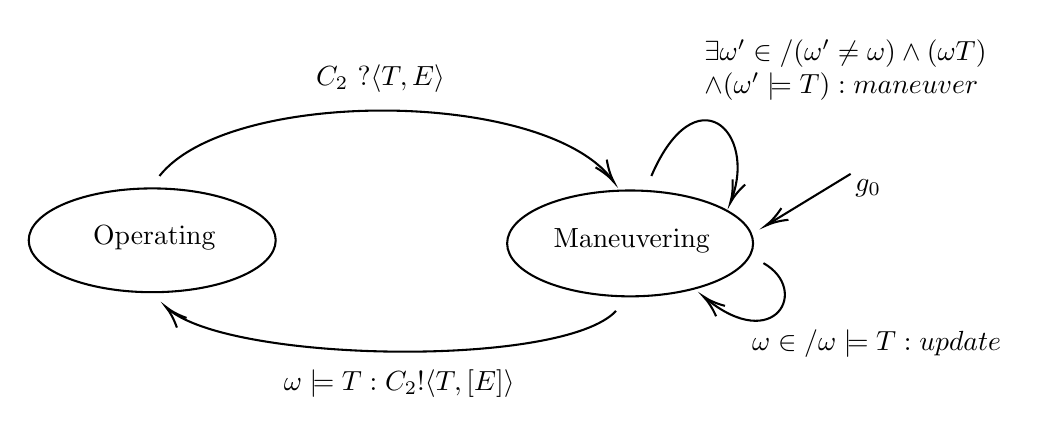
\begin{tikzpicture}[x=0.75pt,y=0.75pt,yscale=-1,xscale=1]
%uncomment if require: \path (0,215); %set diagram left start at 0, and has height of 215

%Curve Lines [id:da9480858267519683] 
\draw    (135.5,88) .. controls (169.16,45.43) and (320.43,45.98) .. (353.53,89.66) ;
\draw [shift={(354.5,91)}, rotate = 235.44] [color={rgb, 255:red, 0; green, 0; blue, 0 }  ][line width=0.75]    (10.93,-3.29) .. controls (6.95,-1.4) and (3.31,-0.3) .. (0,0) .. controls (3.31,0.3) and (6.95,1.4) .. (10.93,3.29)   ;

%Shape: Ellipse [id:dp6594609066072359] 
\draw   (72.5,119) .. controls (72.5,105.19) and (99.14,94) .. (132,94) .. controls (164.86,94) and (191.5,105.19) .. (191.5,119) .. controls (191.5,132.81) and (164.86,144) .. (132,144) .. controls (99.14,144) and (72.5,132.81) .. (72.5,119) -- cycle ;
%Shape: Ellipse [id:dp873836537729809] 
\draw   (303,120.5) .. controls (303,106.42) and (329.53,95) .. (362.25,95) .. controls (394.97,95) and (421.5,106.42) .. (421.5,120.5) .. controls (421.5,134.58) and (394.97,146) .. (362.25,146) .. controls (329.53,146) and (303,134.58) .. (303,120.5) -- cycle ;
%Curve Lines [id:da3135064064897334] 
\draw    (355.5,153) .. controls (329.89,180.58) and (170.39,178.08) .. (139.81,152.2) ;
\draw [shift={(138.5,151)}, rotate = 405] [color={rgb, 255:red, 0; green, 0; blue, 0 }  ][line width=0.75]    (10.93,-3.29) .. controls (6.95,-1.4) and (3.31,-0.3) .. (0,0) .. controls (3.31,0.3) and (6.95,1.4) .. (10.93,3.29)   ;

%Curve Lines [id:da21020703050779688] 
\draw    (372.5,88) .. controls (393.68,38.75) and (423.59,66.15) .. (411.1,99.47) ;
\draw [shift={(410.5,101)}, rotate = 292.38] [color={rgb, 255:red, 0; green, 0; blue, 0 }  ][line width=0.75]    (10.93,-3.29) .. controls (6.95,-1.4) and (3.31,-0.3) .. (0,0) .. controls (3.31,0.3) and (6.95,1.4) .. (10.93,3.29)   ;

%Curve Lines [id:da14662580418826565] 
\draw    (426.5,130) .. controls (449.16,142.81) and (432.03,174.04) .. (399.02,147.26) ;
\draw [shift={(397.5,146)}, rotate = 400.46000000000004] [color={rgb, 255:red, 0; green, 0; blue, 0 }  ][line width=0.75]    (10.93,-3.29) .. controls (6.95,-1.4) and (3.31,-0.3) .. (0,0) .. controls (3.31,0.3) and (6.95,1.4) .. (10.93,3.29)   ;

%Straight Lines [id:da37650774099478246] 
\draw    (468.5,87) -- (429.21,110.96) ;
\draw [shift={(427.5,112)}, rotate = 328.63] [color={rgb, 255:red, 0; green, 0; blue, 0 }  ][line width=0.75]    (10.93,-3.29) .. controls (6.95,-1.4) and (3.31,-0.3) .. (0,0) .. controls (3.31,0.3) and (6.95,1.4) .. (10.93,3.29)   ;


% Text Node
\draw (133,118) node  [align=left] {Operating};
% Text Node
\draw (363,119) node  [align=left] {Maneuvering};
% Text Node
\draw (242,41) node   {$C_{2} \ ?\langle T,E\rangle $};
% Text Node
\draw (251,188) node   {$\omega \models T:C_{2} !\langle T,[ E] \rangle $};
% Text Node
\draw (477,94) node   {$g_{0}$};
% Text Node
\draw (481,169) node   {$\nexists \omega \in \si{\ohm}/\omega \models T:update$};
% Text Node
\draw (466,37) node   {$ \begin{array}{l}
\exists \omega '\in \si{\ohm}/( \omega '\neq \omega ) \land ( \omega \nvDash T)\\
\land ( \omega '\models T) :maneuver
\end{array}$};


\end{tikzpicture}
\label{c2a}
\caption{C2 Approach selector PG}
\end{figure}

\begin{enumerate}
    \item $g_0=\{\omega\in\Omega,T\subseteq M\} $
    
    \item $Loc=\{Operating, Maneuvering\} $
    
    \item $Loc_0=\{Maneuvering\} $
    
    \item $Var=\{find\_maneuver(\omega,\{E\},T), f\_remove(T), \omega, T, E\} $
    
    \item $Cap(C_2)=0 $
    
    \item $\Omega=\{Edge, De-Conflicted, Coord, Conflicted, Collab \}$
    
\end{enumerate}

The effects caused by the actions are defined by

    \qquad $Effect(maneuver, \eta)= \eta[\omega:= find\_maneuver(\omega, \{E\}, T)]$
    
    \qquad $Effect(update, \eta): \eta[T:=f\_remove(T)]$
    


The $f\_remove$ function is responsible to generate a $T' \subseteq T$ such that 

\begin{center}
$ \exists \omega \in \Omega / \omega \models T' $
\end{center}

We can list the following property of the PG presented in \ref{pg01}:

\begin{center}
$ \square (\diamond Operating) $
\end{center}

Task Allocator role is represented by the PG in Figure \ref{ta} where

\begin{enumerate}

    \item $Loc=\{C2A Selecting, Idle, Updating, Allocating, Binding, Notifying \}$
    
    \item $Loc_0=\{Idle\}$
    
    \item $Var=\{alloc, f\_alloc, T, E, t\} $
    
    \item $Cap(C_2)=0 $
    
    \item $Cap(C_1)>0 $
    
    \item $Cap(m_k)>0 $
    
    \item $alloc=\{\langle k,T \rangle\}  $
\end{enumerate}

$k$ variable represents the index of the element $E$ in the set of all agents ($\{E\}$) and it is in the interval $[1..|\{E\}|]$ . T is a set of tasks $t$. The effects of the actions are defined by:

\qquad $Effect(allocate, \eta)= \eta[alloc:= f\_alloc(T, \{E\})]$
    
\qquad $Effect(bind, \eta): \eta[\langle k,T \rangle:=head(alloc); alloc:=tail(alloc)]$

\begin{figure}[h]
\centering
\begin{center}
\end{center}
\begin{center}
\end{center}



\tikzset{every picture/.style={line width=0.75pt}} %set default line width to 0.75pt        

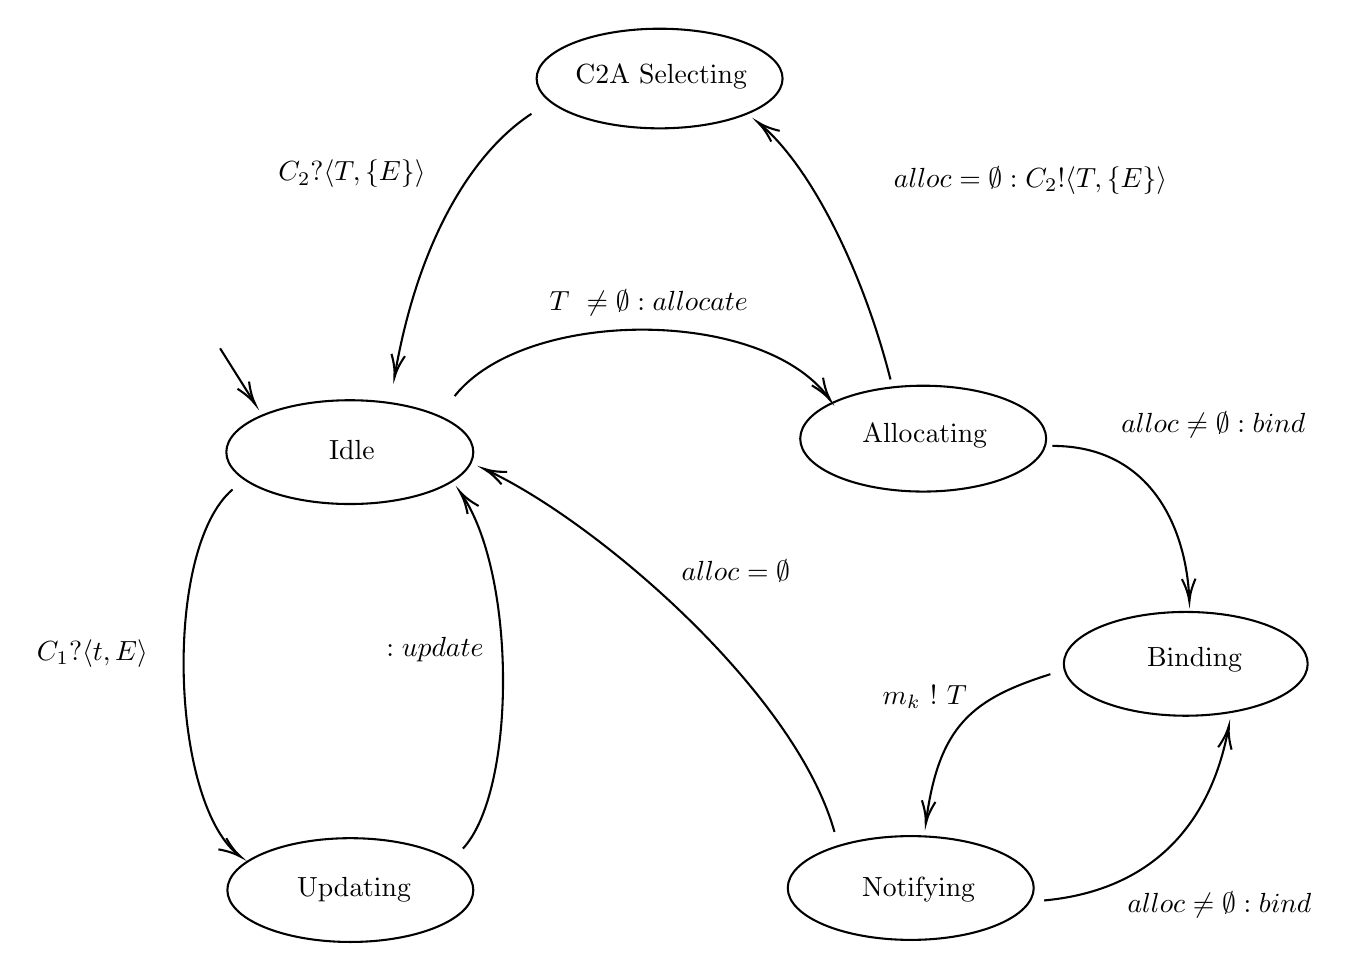
\begin{tikzpicture}[x=0.75pt,y=0.75pt,yscale=-1,xscale=1]
%uncomment if require: \path (0,455); %set diagram left start at 0, and has height of 455

%Curve Lines [id:da9480858267519683] 
\draw    (230.5,181) .. controls (264.16,138.43) and (378.19,138) .. (410.54,181.66) ;
\draw [shift={(411.5,183)}, rotate = 235.44] [color={rgb, 255:red, 0; green, 0; blue, 0 }  ][line width=0.75]    (10.93,-3.29) .. controls (6.95,-1.4) and (3.31,-0.3) .. (0,0) .. controls (3.31,0.3) and (6.95,1.4) .. (10.93,3.29)   ;

%Shape: Ellipse [id:dp6594609066072359] 
\draw   (120.5,208) .. controls (120.5,194.19) and (147.14,183) .. (180,183) .. controls (212.86,183) and (239.5,194.19) .. (239.5,208) .. controls (239.5,221.81) and (212.86,233) .. (180,233) .. controls (147.14,233) and (120.5,221.81) .. (120.5,208) -- cycle ;
%Shape: Ellipse [id:dp873836537729809] 
\draw   (397,201.5) .. controls (397,187.42) and (423.53,176) .. (456.25,176) .. controls (488.97,176) and (515.5,187.42) .. (515.5,201.5) .. controls (515.5,215.58) and (488.97,227) .. (456.25,227) .. controls (423.53,227) and (397,215.58) .. (397,201.5) -- cycle ;
%Curve Lines [id:da14662580418826565] 
\draw    (514.5,424) .. controls (567.96,419.05) and (594.96,385.68) .. (603.25,341.35) ;
\draw [shift={(603.5,340)}, rotate = 460.08] [color={rgb, 255:red, 0; green, 0; blue, 0 }  ][line width=0.75]    (10.93,-3.29) .. controls (6.95,-1.4) and (3.31,-0.3) .. (0,0) .. controls (3.31,0.3) and (6.95,1.4) .. (10.93,3.29)   ;

%Straight Lines [id:da37650774099478246] 
\draw    (117.5,158) -- (133.43,183.31) ;
\draw [shift={(134.5,185)}, rotate = 237.8] [color={rgb, 255:red, 0; green, 0; blue, 0 }  ][line width=0.75]    (10.93,-3.29) .. controls (6.95,-1.4) and (3.31,-0.3) .. (0,0) .. controls (3.31,0.3) and (6.95,1.4) .. (10.93,3.29)   ;

%Shape: Ellipse [id:dp8139093405894636] 
\draw   (121,419) .. controls (121,405.19) and (147.53,394) .. (180.25,394) .. controls (212.97,394) and (239.5,405.19) .. (239.5,419) .. controls (239.5,432.81) and (212.97,444) .. (180.25,444) .. controls (147.53,444) and (121,432.81) .. (121,419) -- cycle ;
%Shape: Ellipse [id:dp08678607998247811] 
\draw   (391,418) .. controls (391,404.19) and (417.53,393) .. (450.25,393) .. controls (482.97,393) and (509.5,404.19) .. (509.5,418) .. controls (509.5,431.81) and (482.97,443) .. (450.25,443) .. controls (417.53,443) and (391,431.81) .. (391,418) -- cycle ;
%Shape: Ellipse [id:dp07482494496489733] 
\draw   (270,28) .. controls (270,14.75) and (296.53,4) .. (329.25,4) .. controls (361.97,4) and (388.5,14.75) .. (388.5,28) .. controls (388.5,41.25) and (361.97,52) .. (329.25,52) .. controls (296.53,52) and (270,41.25) .. (270,28) -- cycle ;
%Curve Lines [id:da6759956440889884] 
\draw    (123.5,226) .. controls (90.01,254.57) and (93.39,375.3) .. (125.99,401.85) ;
\draw [shift={(127.5,403)}, rotate = 215.22] [color={rgb, 255:red, 0; green, 0; blue, 0 }  ][line width=0.75]    (10.93,-3.29) .. controls (6.95,-1.4) and (3.31,-0.3) .. (0,0) .. controls (3.31,0.3) and (6.95,1.4) .. (10.93,3.29)   ;

%Curve Lines [id:da9572857730465772] 
\draw    (234.22,228.76) .. controls (260.49,268.16) and (260.11,371.42) .. (234.5,399) ;

\draw [shift={(233,227)}, rotate = 54.11] [color={rgb, 255:red, 0; green, 0; blue, 0 }  ][line width=0.75]    (10.93,-3.29) .. controls (6.95,-1.4) and (3.31,-0.3) .. (0,0) .. controls (3.31,0.3) and (6.95,1.4) .. (10.93,3.29)   ;
%Curve Lines [id:da9385545433271328] 
\draw    (517.5,315) .. controls (479.88,326.88) and (463.82,339.74) .. (457.68,385.6) ;
\draw [shift={(457.5,387)}, rotate = 277.28] [color={rgb, 255:red, 0; green, 0; blue, 0 }  ][line width=0.75]    (10.93,-3.29) .. controls (6.95,-1.4) and (3.31,-0.3) .. (0,0) .. controls (3.31,0.3) and (6.95,1.4) .. (10.93,3.29)   ;

%Curve Lines [id:da13526468384837043] 
\draw    (440.5,173) .. controls (426.78,119.1) and (401.54,70) .. (377.94,50.18) ;
\draw [shift={(376.5,49)}, rotate = 398.37] [color={rgb, 255:red, 0; green, 0; blue, 0 }  ][line width=0.75]    (10.93,-3.29) .. controls (6.95,-1.4) and (3.31,-0.3) .. (0,0) .. controls (3.31,0.3) and (6.95,1.4) .. (10.93,3.29)   ;

%Curve Lines [id:da7876400787103589] 
\draw    (267.5,45) .. controls (238.79,63.81) and (213.02,106.14) .. (201.83,170.06) ;
\draw [shift={(201.5,172)}, rotate = 279.61] [color={rgb, 255:red, 0; green, 0; blue, 0 }  ][line width=0.75]    (10.93,-3.29) .. controls (6.95,-1.4) and (3.31,-0.3) .. (0,0) .. controls (3.31,0.3) and (6.95,1.4) .. (10.93,3.29)   ;

%Shape: Ellipse [id:dp538933115831977] 
\draw   (524,310) .. controls (524,296.19) and (550.3,285) .. (582.75,285) .. controls (615.2,285) and (641.5,296.19) .. (641.5,310) .. controls (641.5,323.81) and (615.2,335) .. (582.75,335) .. controls (550.3,335) and (524,323.81) .. (524,310) -- cycle ;
%Curve Lines [id:da663291454681702] 
\draw    (518.5,205) .. controls (566.52,205) and (582.85,245.34) .. (584.42,278.01) ;
\draw [shift={(584.5,280)}, rotate = 268.26] [color={rgb, 255:red, 0; green, 0; blue, 0 }  ][line width=0.75]    (10.93,-3.29) .. controls (6.95,-1.4) and (3.31,-0.3) .. (0,0) .. controls (3.31,0.3) and (6.95,1.4) .. (10.93,3.29)   ;

%Curve Lines [id:da17641910717404863] 
\draw    (413.5,391) .. controls (394.69,323.68) and (299.43,241.66) .. (246.1,216.74) ;
\draw [shift={(244.5,216)}, rotate = 384.36] [color={rgb, 255:red, 0; green, 0; blue, 0 }  ][line width=0.75]    (10.93,-3.29) .. controls (6.95,-1.4) and (3.31,-0.3) .. (0,0) .. controls (3.31,0.3) and (6.95,1.4) .. (10.93,3.29)   ;


% Text Node
\draw (181,207) node  [align=left] {Idle};
% Text Node
\draw (457,200) node  [align=left] {Allocating};
% Text Node
\draw (324,136) node   {$T\ \neq \emptyset :allocate$};
% Text Node
\draw (182,419) node  [align=left] {Updating};
% Text Node
\draw (454,419) node  [align=left] {Notifying};
% Text Node
\draw (330,27) node  [align=left] {C2A Selecting};
% Text Node
\draw (56,305) node   {$C_{1} ?\langle t,E\rangle $};
% Text Node
\draw (221,303) node   {$:update$};
% Text Node
\draw (508,77) node   {$alloc=\emptyset :C_{2} !\langle T,\{E\} \rangle $};
% Text Node
\draw (181,74) node   {$C_{2} ?\langle T,\{E\} \rangle $};
% Text Node
\draw (587,308) node  [align=left] {Binding};
% Text Node
\draw (599,426) node   {$alloc\neq \emptyset :bind$};
% Text Node
\draw (457,326) node   {$m_{k\ } !\ T$};
% Text Node
\draw (596,195) node   {$alloc\neq \emptyset :bind$};
% Text Node
\draw (366,265) node   {$alloc=\emptyset $};


\end{tikzpicture}
\label{ta}
\caption{Task Allocator PG}
\end{figure}

Property: 

\begin{center}
$ \square (\diamond Idle) $
\end{center}

The task allocator will be called by the task executor, that is defined by the program graph in Figure \ref{executor}.

\begin{figure}[h]
\centering
\begin{center}
\end{center}
\begin{center}
\end{center}
\begin{center}
\end{center}



\tikzset{every picture/.style={line width=0.75pt}} %set default line width to 0.75pt        

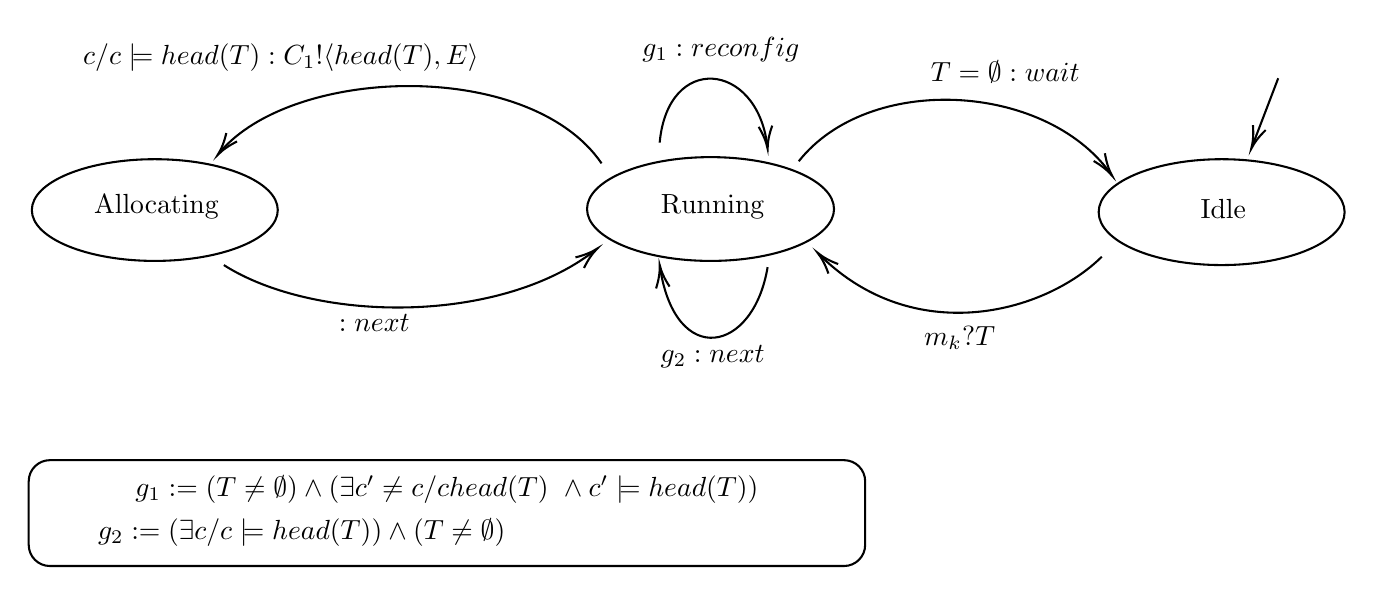
\begin{tikzpicture}[x=0.75pt,y=0.75pt,yscale=-1,xscale=1]
%uncomment if require: \path (0,306); %set diagram left start at 0, and has height of 306

%Curve Lines [id:da9480858267519683] 
\draw    (379.5,108) .. controls (413.16,65.43) and (497.79,69.9) .. (529.55,113.66) ;
\draw [shift={(530.5,115)}, rotate = 235.44] [color={rgb, 255:red, 0; green, 0; blue, 0 }  ][line width=0.75]    (10.93,-3.29) .. controls (6.95,-1.4) and (3.31,-0.3) .. (0,0) .. controls (3.31,0.3) and (6.95,1.4) .. (10.93,3.29)   ;

%Shape: Ellipse [id:dp6594609066072359] 
\draw   (277.5,131) .. controls (277.5,117.19) and (304.14,106) .. (337,106) .. controls (369.86,106) and (396.5,117.19) .. (396.5,131) .. controls (396.5,144.81) and (369.86,156) .. (337,156) .. controls (304.14,156) and (277.5,144.81) .. (277.5,131) -- cycle ;
%Shape: Ellipse [id:dp873836537729809] 
\draw   (524,132.5) .. controls (524,118.42) and (550.53,107) .. (583.25,107) .. controls (615.97,107) and (642.5,118.42) .. (642.5,132.5) .. controls (642.5,146.58) and (615.97,158) .. (583.25,158) .. controls (550.53,158) and (524,146.58) .. (524,132.5) -- cycle ;
%Curve Lines [id:da3135064064897334] 
\draw    (364.5,159) .. controls (357.57,200.58) and (320.26,207.86) .. (312.72,159.48) ;
\draw [shift={(312.5,158)}, rotate = 442.03] [color={rgb, 255:red, 0; green, 0; blue, 0 }  ][line width=0.75]    (10.93,-3.29) .. controls (6.95,-1.4) and (3.31,-0.3) .. (0,0) .. controls (3.31,0.3) and (6.95,1.4) .. (10.93,3.29)   ;

%Curve Lines [id:da21020703050779688] 
\draw    (312.5,99) .. controls (316.44,55.66) and (359.19,59.86) .. (364.29,100.14) ;
\draw [shift={(364.5,102)}, rotate = 264.56] [color={rgb, 255:red, 0; green, 0; blue, 0 }  ][line width=0.75]    (10.93,-3.29) .. controls (6.95,-1.4) and (3.31,-0.3) .. (0,0) .. controls (3.31,0.3) and (6.95,1.4) .. (10.93,3.29)   ;

%Straight Lines [id:da37650774099478246] 
\draw    (610.5,68) -- (598.21,100.13) ;
\draw [shift={(597.5,102)}, rotate = 290.92] [color={rgb, 255:red, 0; green, 0; blue, 0 }  ][line width=0.75]    (10.93,-3.29) .. controls (6.95,-1.4) and (3.31,-0.3) .. (0,0) .. controls (3.31,0.3) and (6.95,1.4) .. (10.93,3.29)   ;

%Shape: Ellipse [id:dp02234558999259495] 
\draw   (10,131.5) .. controls (10,117.97) and (36.53,107) .. (69.25,107) .. controls (101.97,107) and (128.5,117.97) .. (128.5,131.5) .. controls (128.5,145.03) and (101.97,156) .. (69.25,156) .. controls (36.53,156) and (10,145.03) .. (10,131.5) -- cycle ;
%Curve Lines [id:da2517277021570281] 
\draw    (284.5,109) .. controls (249.85,58.51) and (135.81,61.93) .. (100.54,103.72) ;
\draw [shift={(99.5,105)}, rotate = 308.33000000000004] [color={rgb, 255:red, 0; green, 0; blue, 0 }  ][line width=0.75]    (10.93,-3.29) .. controls (6.95,-1.4) and (3.31,-0.3) .. (0,0) .. controls (3.31,0.3) and (6.95,1.4) .. (10.93,3.29)   ;

%Curve Lines [id:da851947022127026] 
\draw    (102.5,158) .. controls (146.06,185.72) and (234.7,186.98) .. (281.11,151.1) ;
\draw [shift={(282.5,150)}, rotate = 501.19] [color={rgb, 255:red, 0; green, 0; blue, 0 }  ][line width=0.75]    (10.93,-3.29) .. controls (6.95,-1.4) and (3.31,-0.3) .. (0,0) .. controls (3.31,0.3) and (6.95,1.4) .. (10.93,3.29)   ;

%Curve Lines [id:da05773774536505705] 
\draw    (525.5,154) .. controls (497.29,181.72) and (434.77,197.68) .. (389.86,153.36) ;
\draw [shift={(388.5,152)}, rotate = 405.63] [color={rgb, 255:red, 0; green, 0; blue, 0 }  ][line width=0.75]    (10.93,-3.29) .. controls (6.95,-1.4) and (3.31,-0.3) .. (0,0) .. controls (3.31,0.3) and (6.95,1.4) .. (10.93,3.29)   ;

%Rounded Rect [id:dp5913972444482631] 
\draw   (8.5,262.2) .. controls (8.5,256.57) and (13.07,252) .. (18.7,252) -- (401.3,252) .. controls (406.93,252) and (411.5,256.57) .. (411.5,262.2) -- (411.5,292.8) .. controls (411.5,298.43) and (406.93,303) .. (401.3,303) -- (18.7,303) .. controls (13.07,303) and (8.5,298.43) .. (8.5,292.8) -- cycle ;

% Text Node
\draw (338,130) node  [align=left] {Running};
% Text Node
\draw (584,131) node  [align=left] {Idle};
% Text Node
\draw (479,65) node   {$T=\emptyset :wait$};
% Text Node
\draw (130,58) node   {$\nexists c/c\models head( T) :C_{1} !\langle head( T) ,E\rangle $};
% Text Node
\draw (457,193) node   {$m_{k} ?T$};
% Text Node
\draw (70,130) node  [align=left] {Allocating};
% Text Node
\draw (175,186) node   {$:next$};
% Text Node
\draw (210,266) node   {$g_{1} :=( T\neq \emptyset ) \land ( \exists c'\neq c/c\nvDash head( T) \ \land c'\models head( T))$};
% Text Node
\draw (342,54) node   {$g_{1} :reconfig$};
% Text Node
\draw (338,202) node   {$g_{2} :next$};
% Text Node
\draw (140,287) node   {$g_{2} :=( \exists c/c\models head( T)) \land ( T\neq \emptyset )$};


\end{tikzpicture}
\label{executor}
\caption{Task Executor PG}
\end{figure}

Its elements is listed below:

\begin{enumerate}

    \item $Loc=\{Running, Idle, Allocating \}$
    
    \item $Loc_0=\{Idle\}$
    
    \item $Var=\{T, E, c\} $
    
    \item $Cap(C_1)>0 $
    
    \item $Cap(m_k)>0 $
    
\end{enumerate}

where $k$ indicates the index of the executor in analysis.

The effects of the actions are defined by

\qquad $Effect(reconfig, \eta)= \eta[c:=c']$
    
\qquad $Effect(next, \eta): \eta[T:=tail(T)]$

\qquad $Effect(wait, \eta): \eta$

For the task executor, the following properties can be identified:

\qquad $\square \diamond (Idle)$

\qquad $\diamond Running$